\documentclass[a4paper,papersize,dvipdfmx]{jsarticle}
\usepackage{ascmac}
\usepackage{mathtools, amssymb,bm}
\usepackage{comment}
\usepackage[hiresbb]{graphicx}
\usepackage{tcolorbox,color}
\usepackage{here}
\tcbuselibrary{raster,skins,breakable}

\newcommand{\pic}[1]{\begin{center} \includegraphics[width=1.0\linewidth,clip]{#1} \end{center}}   %写真用
\newcommand{\pict}[2]{\begin{center} \includegraphics[width= {#2} cm]{#1} \end{center}}   %写真用
\newcommand{\redunderline}[1]{\textcolor{red}{\underline{¥textcolor{black}{#1}}}}   %赤いアンダーライン
\newcommand{\mon}[1]{\item[({#1})] \ }
\newcommand{\ctext}[1]{\raise0.2ex\hbox{\textcircled{\scriptsize{#1}}}}%文字を丸囲みする(2桁の数字までならいける)

% 画像を貼る時はjpgかjpegで、pngはうまくいかないっぽい

%\itemを四角で囲った数字にする場合は以下のコメントアウトを消す
%\renewcommand{\labelenumi}{\textbf{\framebox[1.5zw]{\theenumi}}}


%enumerateの2階層めのカウンタを1,2,3, にする時は以下のコメントアウトを消す
\renewcommand{\theenumii}{\arabic{enumii}}

%enumerateのカウンタについては以下を参照
% http://www3.otani.ac.jp/fkdsemi/pLaTeX_manual/kajyo.html


%enumerateの番号の出力形式を変更するには、カウンタの値を出力する命令を定義し直す。
%レベル	カウンタ	出力する命令	デフォルトの出力
%1	enumi	¥theenumi	アラビア数字(1,2,3,・・・)
%2	enumii	¥theenumii	小文字のアルファベット(a,b,c,・・・)
%3	enumiii	¥theenumiii	小文字のローマ数字(小文字のローマ数字(\UTF{2170},\UTF{2171},\UTF{2172},・・・)
%4	enumiv	¥theenumiv	大文字のアルファベット(A,B,C,・・・)
%例:¥enumiカウンタを大文字のローマ数字で出力する設定
% ¥renewcommand{¥theenumi}{¥Roman{enumi}}

% 番号の出力形式
%命令	出力形式
%¥arabic	アラビア数字(1、2、3、・・・)
%¥roman	ローマ数字(\UTF{2170}、\UTF{2171}、\UTF{2172}、・・・)
%¥Roman	ローマ数字(\UTF{2160}、\UTF{2161}、\UTF{2162}、・・・)
%¥alph	アルファベット(a、b、c、・・・)
%¥Alph	アルファベット(A、B、C、・・・)




\begin{document}

\title{実習レポート 天然物化学教室}
\author{10191043 鈴木健一}
%作成日を入れる場合は消す
\date{}
\maketitle

%以下の3つからフォントサイズを選択するとよい
%\footnotesize
%\small
%\normalsize



\begin{flushright}
実験日 : 2019/5/29 $\sim$ 2019/6/3

共同実験者 : 白井孝平
\end{flushright}


\part{Berberineの単離とその化学}

\subsection*{目的}
著名な生薬から重要薬物を単離するために必要とする基礎技術及び分光学的手法、化学的手法による構造解析に習熟する。

\section*{1日目 黄柏よりberberineの単離(1)}
\subsection*{実験方法}
\begin{enumerate}
\item 黄柏を2Lナスフラスコに入れる
\item メタノールを加え75℃で1時間還流する。
\item 40〜50℃に冷まして綿栓濾過を行う
\item エバポレーターで200mLに濃縮する。この時湯浴の温度は40℃程度にする。
\item 水を500mL加えて一日放置する。
\end{enumerate}
\subsection*{結果}
\begin{itemize}
\item 黄柏にメタノールを加えて還流すると液の色が黄色く変化した。

\end{itemize}
\section*{2日目 黄柏よりberberineの単離(2)}
\subsection*{実験方法}
\begin{enumerate}
\item 昨晩放置した黄柏の濾液の不溶物を綿栓濾過で取り除く。
\item 再度ひだ折りろ紙を用いて濾過する
\item エバポレーターで500mLまで濃縮して濾過する。
\item 15\%の塩酸を100mL添加する。
\item 氷冷して結晶化する。
\item 粗結晶をブフナーロートで濾取する。
\item 冷アセトンで十分洗い、湯浴を用いて水に溶かす。
\item 濾液に少量の塩酸を加えて再び結晶化させる。
\item ブフナーロートで濾取し、洗浄後にでしけーターで乾燥する。
\item 融点と重量を測定する。

\end{enumerate}
\subsection*{結果}
\begin{itemize}
\item 重量 : 2.47 g
\item 分解点 : 165℃ (文献値 : 204℃)
\item 融点を測定して結晶が分解すると色が赤褐色に変化した。
\item はじめに氷浴しながら塩酸を加えても全く析出物がなかったので、再び塩酸を加えてスパーテルで内壁を激しくこすると黄色い沈殿が発生した。これを濾過すると黄色い粗結晶が得られた。
\item 再結晶すると結晶が水を吸って大きくなったのでろ紙で水を十分に取り除いてから乾燥した。

\end{itemize}
\subsection*{考察 : 今回の結晶化で塩酸を用いた理由}
溶液内には様々なイオンが溶けているが、塩酸を加えることで陰イオンが塩化物イオンに統一されるので、berberineと塩化物イオンの溶解度積が限界量を超えてberberine clorideの塩がより多く析出する。

\section*{3日目 berberineのdl-canadineへの還元}
\subsection*{実験方法}
\begin{enumerate}
\item 3 gのberberine chlorideを200mLの三角フラスコにとり、60mLのメタノールを加えて水浴上で45℃程度に加熱して溶解させる。
\item 常温に戻したら1.5gの$\rm NaBH_4$を5分以上分けてゆっくりと加えて、1時間静置する。
\item 反応の終結はTLCで確認する。原料の消失を確認したら水30mLを加えさらに30分静置する。
\item 結晶を濾取して少量のメタノールで洗った後、クロロホルムに溶かし、不純物を濾去する。
\item 濾液を濃縮乾固し、残渣を 5〜6mLのクロロホルムに水浴上で加熱しながら溶かし、60mLのメタノールを加え結晶を析出させる。
\item 濾取、乾燥したのちに融点と重量を求める。
\end{enumerate}
\subsection*{結果}
\begin{itemize}
\item berberine chloride にメタノールを加えると黄色い溶液となった。
\item その後白色結晶の$\rm NaBH_4$を1.50 g加えると大量の泡と熱をが生じた。一度溶液が黒く変化したが、下に白い沈殿が発生して溶液の色は黄色に戻った。
\item 最終的には明るいレモン色の結晶が得られたが、本来の結晶の色は白らしい。
\item 収量 : 0.78 g
\item 融点 : 147〜149℃

\end{itemize}
\subsubsection*{TLC}
\begin{figure}[H]
\begin{center}
\begin{tabular}{c}

\begin{minipage}{0.22\hsize}
\begin{center}
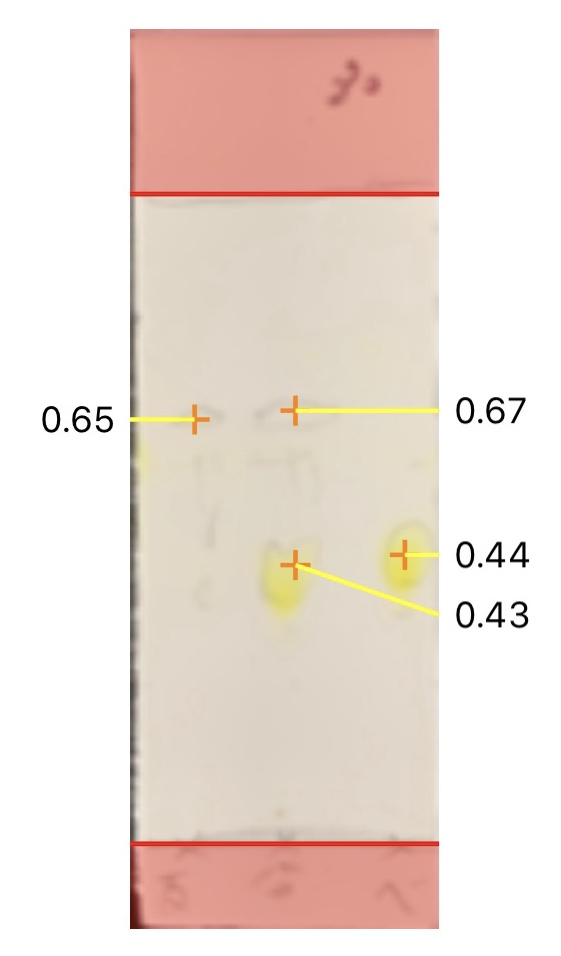
\includegraphics[clip, height=7cm]{imgs/3-tlc1.jpg}
\hspace{1.6cm} 30分
\end{center}
\end{minipage}

\begin{minipage}{0.05\hsize}
\hspace{2mm}
\end{minipage}

\begin{minipage}{0.22\hsize}
\begin{center}
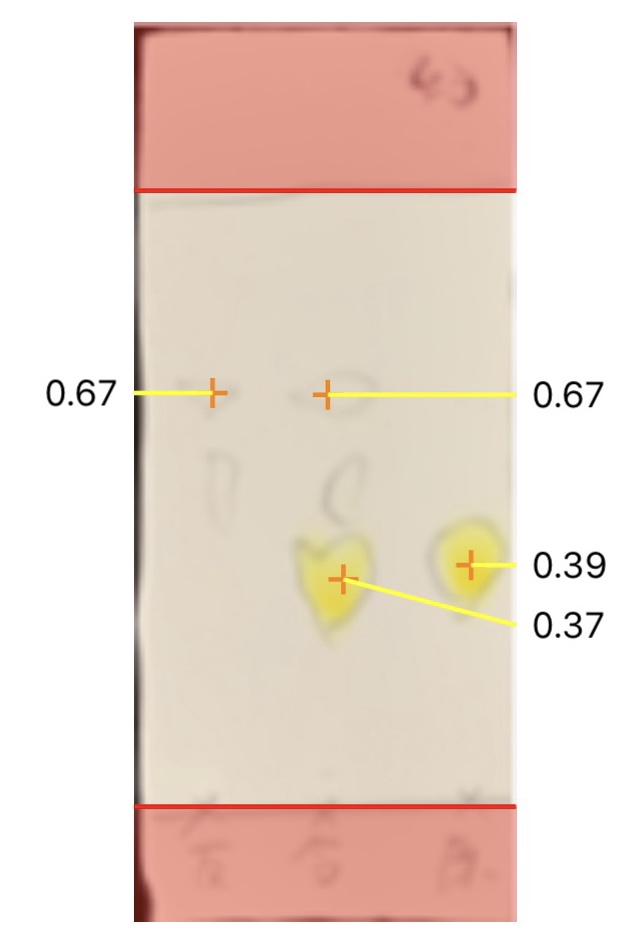
\includegraphics[clip, height=7cm]{imgs/3-tlc2.jpg}
\hspace{1.6cm} 45分
\end{center}
\end{minipage}

\end{tabular}
\end{center}
\end{figure}

\subsection*{考察}
berberine は dl-canadine に比べて共役系が長いため、黄色い蛍光を発していると考えられる。


\section*{問題}

\begin{tcolorbox}[colback=white,colbacktitle=black,coltitle=white,title={問題1}]
\begin{itemize}
\item (1) Berberineの$\rm NaBH_4$による還元のメカニズムを考察せよ
\item (2) Berberine, canadine の生合成について考察せよ
\end{itemize}
\end{tcolorbox}

(1)  Berberineは$\rm NaBH_4$によって以下のように還元される
\pict{imgs/kd01.jpg}{12}

(2)  berberine は以下のように生合成される。全13段階のうち2段階はp450が触媒である。
\pic{imgs/kd02.jpg}

\begin{tcolorbox}[colback=white,colbacktitle=black,coltitle=white,title={問題2}]
硫酸ジメチルは典型的なメチル化剤の一つである。実習書1-18における反応条件下で $dl-\rm canadine$ のなかで求電子的なメチル化を受けるのはどこか。
\end{tcolorbox}

$dl-\rm canadine$ の窒素原子の非共有電子対が求電子的なメチル化を受ける。

\begin{tcolorbox}[colback=white,colbacktitle=black,coltitle=white,title={問題3}]
$dl-\rm canadine$ のメチル化物はクロロホルムに難溶であるため、クロロホルム中で結晶として単離された。すなわち、水には溶け易い性質を持っており、メチル化物は塩の形になっているものと思われる。このメチル化物の構造を推定しなさい。
\end{tcolorbox}

\pict{imgs/kd03.jpeg}{4}

\begin{tcolorbox}[colback=white,colbacktitle=black,coltitle=white,title={問題4}]
このメチル化物をアルカリ性条件下で加熱すると、メチル化物を構成していたカウンターイオンの硫酸イオンがカリウムイオンと会合して脱離し、また同時に塩基がプロトンを奪う。ここでメチル化物はイオン化してない状態へ戻るが、ある結合が切れなければならない。結合が切れる可能性は原料に戻る場合を除いて3通り考えられる。その可能性を示しなさい。
\end{tcolorbox}

\pict{imgs/kd04.jpeg}{12}

\begin{tcolorbox}[colback=white,colbacktitle=black,coltitle=white,title={問題5}]
$\rm ^{13}C$の天然存在比率を理化学辞典などで調べなさい。$dl-\rm canadine$の$\rm M^+ +1, M^+,M^+-1$がどんな原子組成から成り立っているか推測しなさい。
\end{tcolorbox}

天然存在比
\[\rm ^{12}C \ : \  ^{13}C \ = \ 98.93\% : 1.07\%\]


$\rm M^+$がberberine分子イオンであり、$\rm M^+ +1$はそのうちの炭素1つが$\rm ^{13}C$である分子イオンである。$\rm M^+-1$は脱水素ラジカルを起こした分子イオンである。このとき脱水素ラジカルを起こす可能性が高いのは窒素原子の隣の炭素原子である。

\begin{tcolorbox}[colback=white,colbacktitle=black,coltitle=white,title={問題6}]
$dl-\rm canadine$の$\rm M^+ +1$のフラグメントピークは、どのような分子構造か。$dl-\rm canadine$のMassスペクトルにおけるbase peak 164はどのような分子構造か。
\end{tcolorbox}

分子量174のピークがあることから、以下のように分子量338の$\rm M^+-1$フラグメントが分離してbase peak と分子量174のフラグメントが生じたと考えられる。

\pict{imgs/kd06.jpeg}{8}

\begin{tcolorbox}[colback=white,colbacktitle=black,coltitle=white,title={問題7}]
図2-1に示した変換物のMassスペクトルから変換物の分子量を推定しなさい。
\end{tcolorbox}

分子イオンピークが353にあり、メチルラジカルの脱離により338のピークを生じることから、$\rm M^+ -1$フラグメントにメチル基が1つ導入されたと考えられる。したがって変換物の分子量は353と考えられる。

\begin{tcolorbox}[colback=white,colbacktitle=black,coltitle=white,title={問題8}]
図2-3に示した変換物のコンプリートとDEPTのチャートを解析し、$\rm CH_3,CH_2, CH, C$の数を数えなさい。
\end{tcolorbox}

\[\rm CH_3\longrightarrow3,  \ \ CH_2 \longrightarrow4, \ \ CH \longrightarrow 6, \ \ C \longrightarrow 8\]

\begin{tcolorbox}[colback=white,colbacktitle=black,coltitle=white,title={問題9}]
$dl-\rm canadine$と変換物の$\rm ^{13}C-NMR$スペクトルを比較して、大きく変化した点を指摘しなさい。
\end{tcolorbox}

以下に示す$dl-\rm canadine$の5番と6番の炭素に相当するピークが消失している。その代わりに新たなピーク(43.255, 114.593, 134.282)が現れている。

\pict{imgs/kd09.jpeg}{5}

\begin{tcolorbox}[colback=white,colbacktitle=black,coltitle=white,title={問題10}]
問題4で考えた3通り仮想生成物から問題9で指摘した点を最もよく説明するものの構造を示し、その理由を説明せよ。また、メチル化物から変換物が生成する段階は著名な人名反応であるが、その反応名を書きなさい。
\end{tcolorbox}

問9で指摘した点を最も説明できるのは以下に示す反応経路である。この条件であれば、5番と6番の炭素のピークが消失し、代わりに$\delta _c =  114.593, 134.282$が出現したことを説明できる。$\delta _c = 43.255$はN-メチル化によるものである。また、このように4級アンモニウム塩からプロトンが脱離してアミンとアルケンを生じる反応をホフマン脱離という。

\pict{imgs/kd10.jpeg}{10}

\newpage

\part{Curcuminの単離および生合成酵素を用いた異種生産}

\subsection*{目的}
生合成研究の一例としてCurcumin生合成酵素の酵素化学的研究法の一端に触れる。
\section*{4日目}
\subsection*{実験方法}
\subsubsection*{秋ウコンからクルクミンの単離・精製}
\begin{enumerate}
\item 20gの秋ウコン粉末をいれた100mLの三角フラスコに50mLのジクロロメタンを入れ、60分静置する。得られた抽出液をひだ折りろ紙で濾過し、濾液をエバポレーターで濃縮する。
\item 得られたオイルに対して20mLのヘキサンを加えて析出した固体を桐山ロートで濾取する。
\item ジクロロメタンに溶解させてTLCで分析する。

\end{enumerate}
\subsubsection*{大腸菌を用いたビスデメトキシクルクミンの生産}
ネガティブコントロールとクルクミン生産大腸菌の培養液(10mL)をそれぞれ遠心チューブに入れ、6MHClでpHを約3としたあと、酢酸エチルで抽出(10mL $\times$ 2)する。HClを加える際には発泡がともなうため、様子を見ながら徐々に加える。遠心して酢酸エチル層と水層を分離したあと、酢酸エチル層を取り、$\rm Na_2SO_4$で乾燥後、エバポレーターで濃縮乾固する。残渣を少量のジクロロメタンに溶解し、TLC上にスポットして、ネガティブコントロール、標品と比較することで、ビスデメトキシクルクミンの生産を確認する。

\subsection*{結果}

\subsubsection*{TLC}
\begin{figure}[H]
\begin{center}
\begin{tabular}{c}
\begin{minipage}{0.22\hsize}
\begin{center}
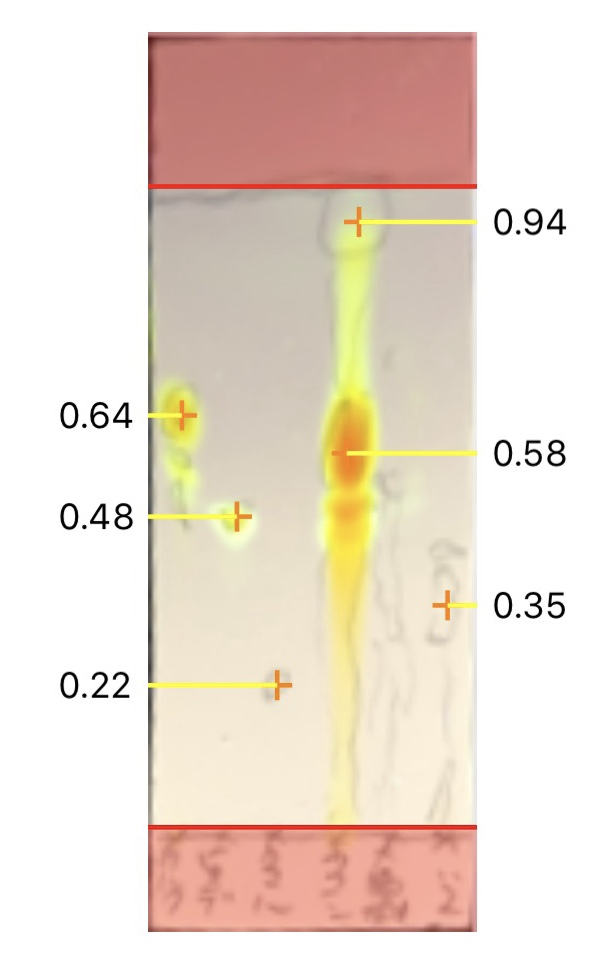
\includegraphics[clip, height=6cm]{imgs/4-tlc1.jpg}

\end{center}
\end{minipage}
\begin{minipage}{0.05\hsize}
\hspace{2mm}
\end{minipage}
\begin{minipage}{0.22\hsize}
\begin{center}
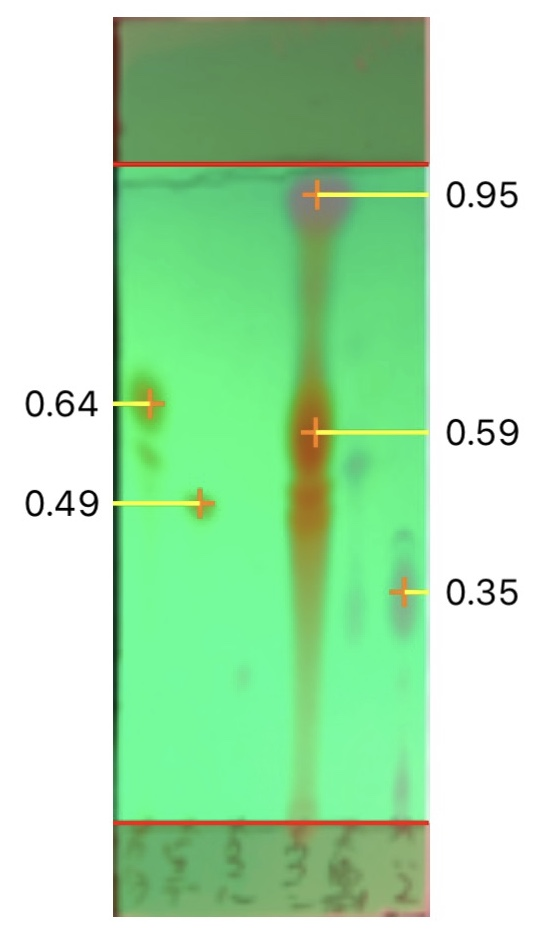
\includegraphics[clip, height=6cm]{imgs/4-tlc2.jpg}

\end{center}
\end{minipage}
\end{tabular}
\end{center}
\end{figure}



\section*{問題}
\begin{tcolorbox}[colback=white,colbacktitle=black,coltitle=white,title={問題1}]
Curcumin の生物活性について述べなさい。また、curcuminと類似の過程により生合成されると予想される天然物を示しなさい。
\end{tcolorbox}

Curcumin は以下のような生物活性を持つ。
\begin{itemize}
\item アミロイド$\beta$凝集抑制
\item 抗炎症
\item 抗がん
\item 脂質代謝改善
\item 抗酸化
\end{itemize}

curcuminと類似の過程により生合成されると予想される天然物はショウガに含まれる成分であるジンゲロンやショウガオールである。

\begin{tcolorbox}[colback=white,colbacktitle=black,coltitle=white,title={問題2}]
CUSの副生成物として、360 nmに極大吸収を示す化合物も生産される。これは実習書の序で述べたCHSの副生成物でもあり、マロニルCoA 2分子の縮合の後に環化を経て生成する。どんな化合物が考えられるか考察しなさい。
\end{tcolorbox}

以下のようにしてcurcuminoids と副生成物の triketide pyrone が生成する。

\pic{imgs/kd22.jpg}

\begin{tcolorbox}[colback=white,colbacktitle=black,coltitle=white,title={問題3}]
ウコンからの抽出・精製と異種発現系によって得られたクルクミノイドについて相違を考察するとともに、大腸菌などの異種発現系を用いた物質生産の利点と欠点を述べなさい。
\end{tcolorbox}

大腸菌は以下のようにしてcurcuminoidsを合成する。
\pict{imgs/kd23.jpeg}{15}

問題2のクルクミノイド合成と比較すると、ウコンでの合成経路では副生成物が生じるが大腸菌では副生成物が生じることがわかる。異種発現系では目的の生成物を特異的に合成することができるという利点がある。しかし、大腸菌では原料が合成できないため、原料を与える必要があるという欠点がある。



\end{document}